% AnatoPhaseNet v7 methodology. Compile with pdflatex (e.g. Overleaf); keep the PNG figures in the same folder.
\documentclass[conference]{IEEEtran}
\usepackage{cite}
\usepackage{amsmath,amssymb}
\usepackage{graphicx}
\usepackage{booktabs}
\usepackage{array}
\usepackage{algorithm}
\usepackage{algpseudocode}
\usepackage[hidelinks]{hyperref}

\begin{document}

\title{AnatoPhaseNet: Phase-Aligned Anatomical Spatio-Temporal Network for Subject-Independent Pathological Gait Classification from Silhouettes}
\author{\IEEEauthorblockN{Shaswati Mishra (123EC0564)}
\IEEEauthorblockA{Department of Electronics and Communication Engineering, National Institute of Technology, Rourkela\\
Supervisor: Prof. Samit Ari}}
\maketitle

\begin{figure*}[t]
\centering
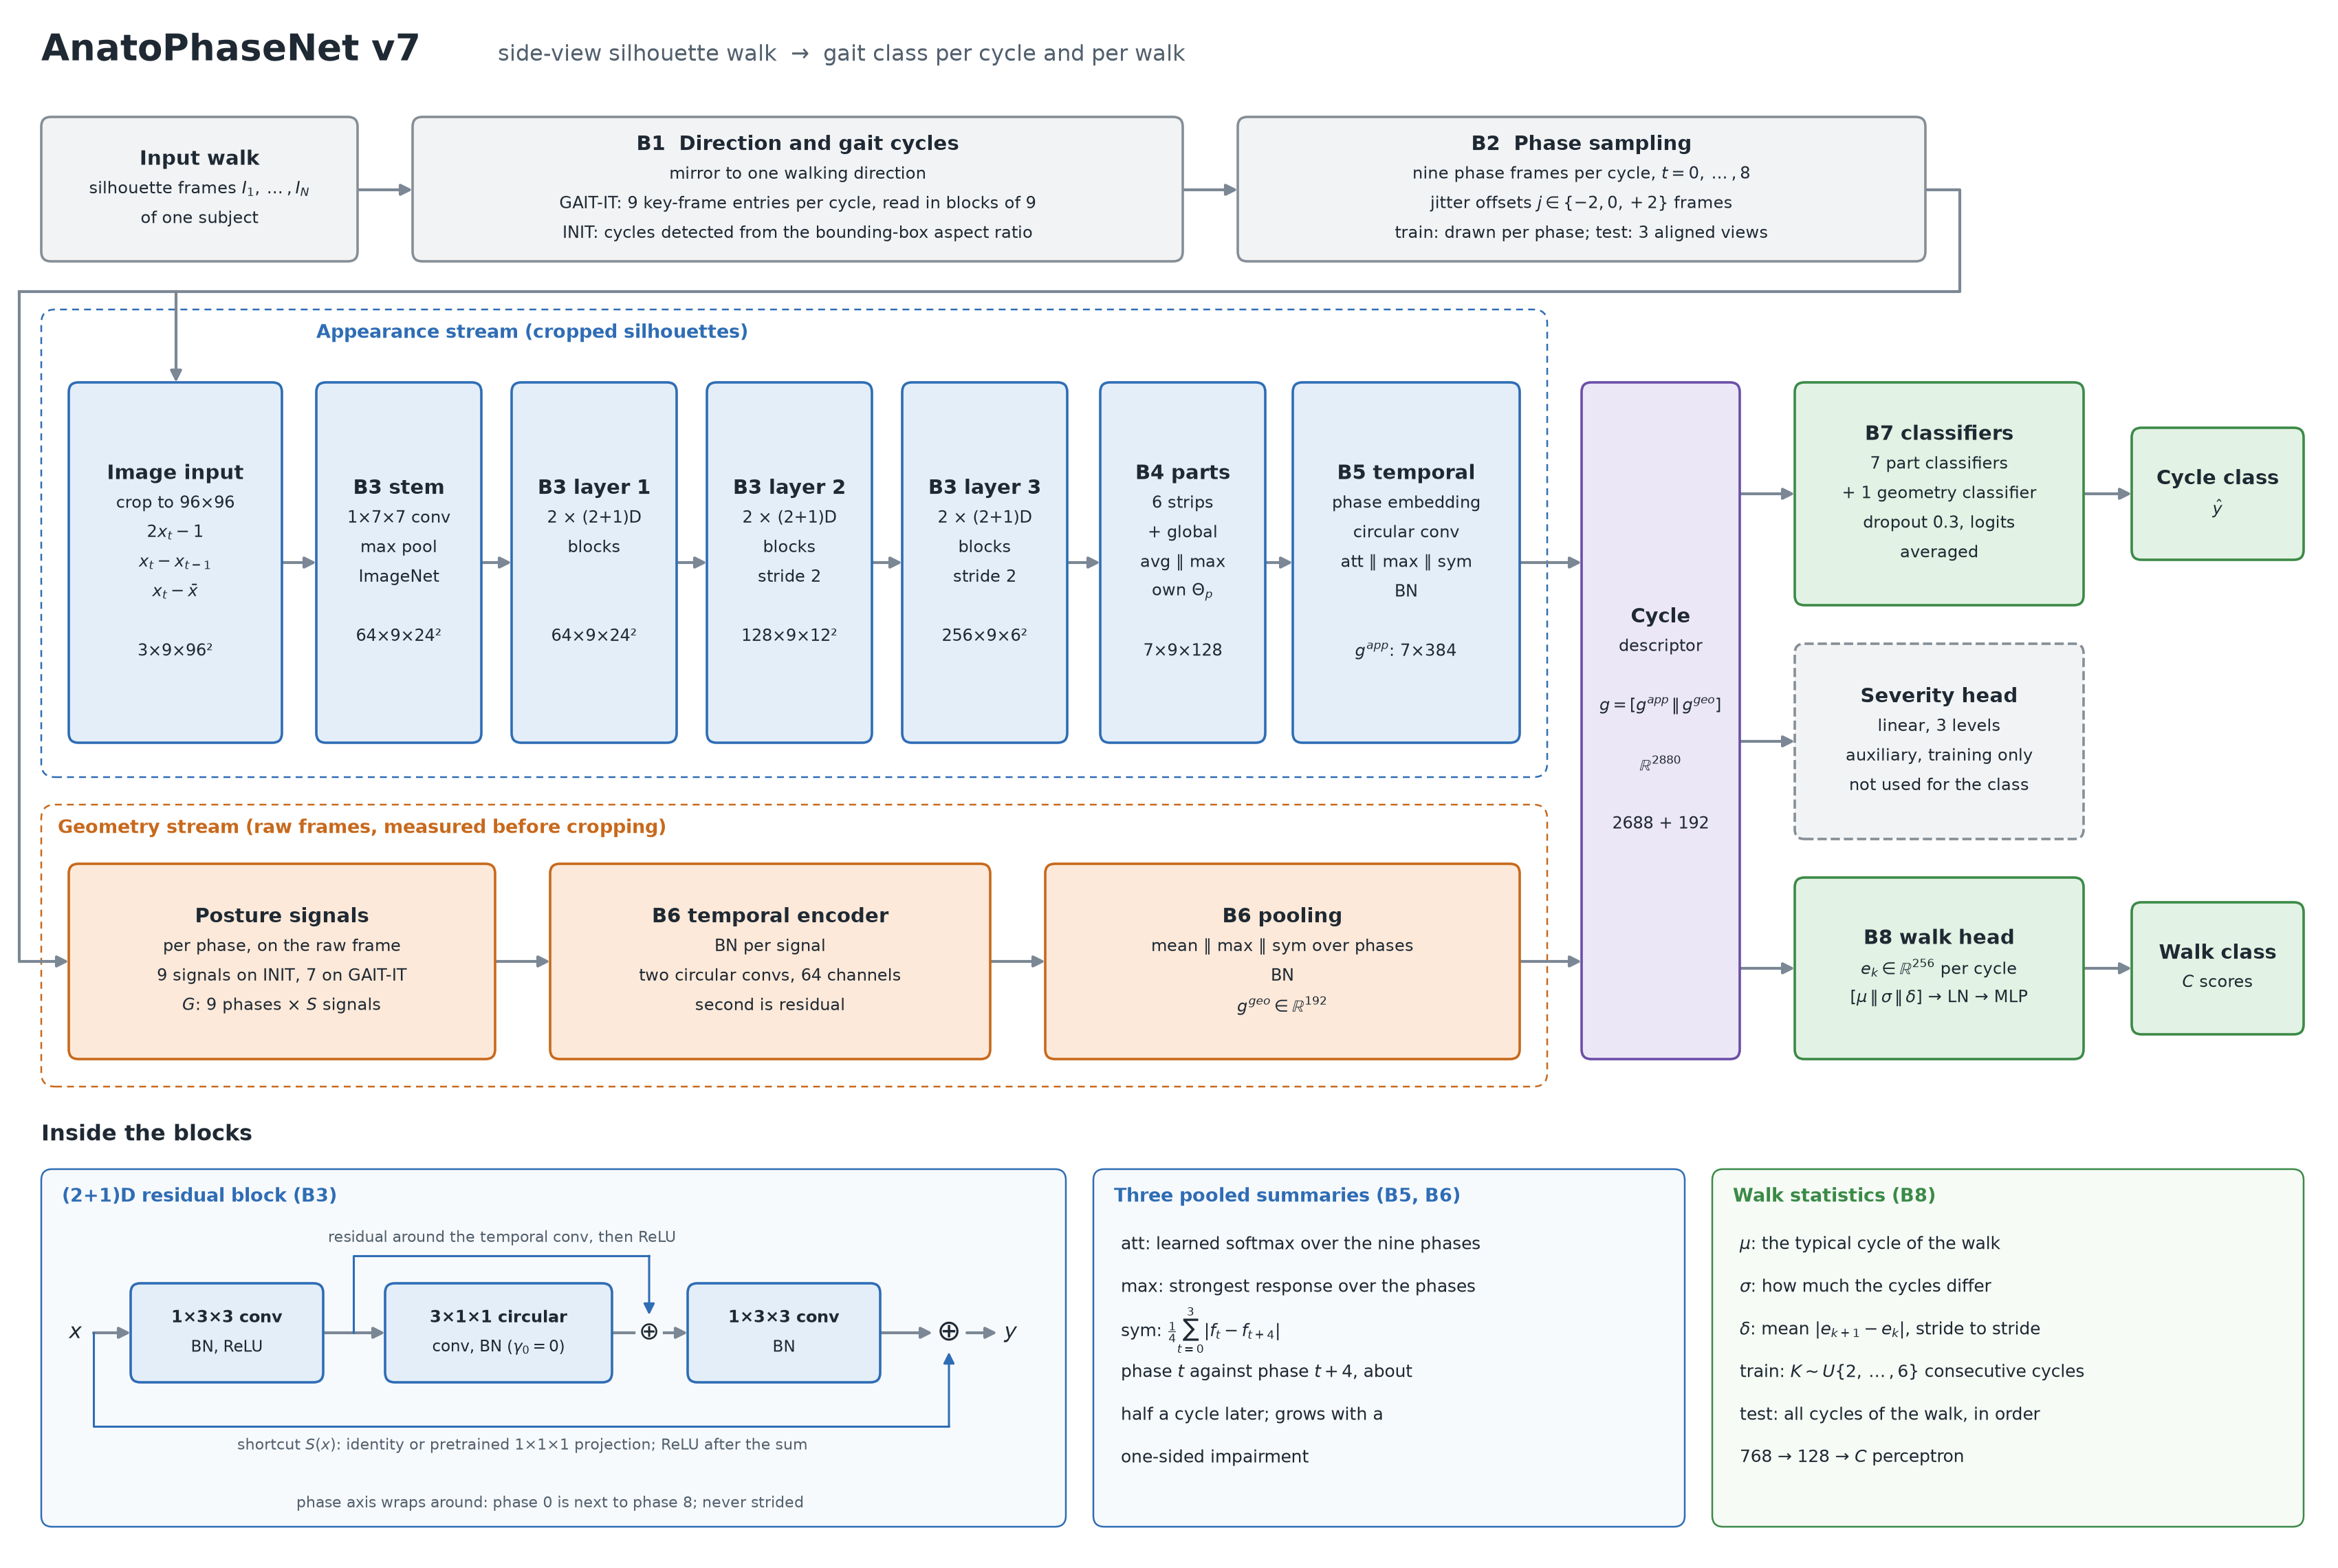
\includegraphics[width=\textwidth]{architecture_v7.png}
\caption{Architecture of AnatoPhaseNet v7. B1--B2 turn a walk into phase-sampled gait cycles. The appearance stream (blue) reads cropped silhouettes; the geometry stream (orange) reads posture signals measured on the raw frames. Their features form the cycle descriptor $\mathbf{g}$, which feeds the cycle classifiers (B7), the walk head (B8) and an auxiliary severity head. The lower panels open the (2+1)D block, the pooled summaries and the walk statistics.}
\label{fig:arch}
\end{figure*}

\section{Methodology}

AnatoPhaseNet assigns a gait class to a person it has not seen, from a side-view silhouette video, and it decides twice: for every gait cycle and for the whole walk. Fig.~\ref{fig:arch} outlines the pipeline. The walk is brought to one walking direction and cut into gait cycles (B1), and each cycle is reduced to nine frames taken at fixed phases of the cycle (B2). These frames feed two streams. The appearance stream (B3--B5) reads the cropped silhouettes body part by body part, and the geometry stream (B6) measures posture on the frames as they were recorded, before our crop. Eight classifiers on the two streams are averaged into the cycle decision (B7), and a walk head (B8) reads several cycles of the same walk together. This section defines version 7 of the model, its training and its evaluation, following the code in \texttt{anato\_phasenet\_v7.py}. Section~\ref{sec:changes} lists what changed from version 6.

\subsection{Problem formulation}

A walk is a sequence of silhouette frames $W=(I_1,\dots,I_N)$ of one subject, filmed from the side, with a gait label $y\in\{1,\dots,C\}$. On GAIT-IT~\cite{gaitit}, $C=5$: normal, diplegic, hemiplegic, neuropathic and Parkinson's gait. On INIT~\cite{init}, $C=6$: normal walking, reduced arm swing on the left or on the right (each merging two levels), a half step with the left or the right leg, and full-body impairment. Table~\ref{tab:data} gives the size of both datasets. B1 cuts $W$ into $M$ gait cycles, and B2 turns cycle $m$ into an image tensor $\mathbf{X}_m$ and a posture matrix $\mathbf{G}_m$. The cycle model $f$ returns class scores and a cycle descriptor,
\begin{equation}
(\mathbf{z}_m,\mathbf{g}_m)=f(\mathbf{X}_m,\mathbf{G}_m),\quad \mathbf{z}_m\in\mathbb{R}^{C},\quad \mathbf{g}_m\in\mathbb{R}^{2880},
\label{eq:model}
\end{equation}
and the walk model $h$ maps the descriptors of a walk's cycles to walk scores $\hat{\mathbf{z}}=h(\mathbf{g}_1,\dots,\mathbf{g}_M)$. Training and test subjects are always disjoint (Section~\ref{sec:eval}), so $f$ and $h$ must recognize a pathology in a person whose build, clothing and walking style they have not seen.

\begin{table}[t]
\centering
\caption{Data Used by the Final Model}
\label{tab:data}
\begin{tabular}{lrrrr}
\toprule
Class & Subjects & Walks & Cycles & Severity levels \\
\midrule
\multicolumn{5}{l}{\textit{GAIT-IT}} \\
Normal & 23 & 92 & 202 & normal \\
Diplegic & 22 & 176 & 846 & mild, severe \\
Hemiplegic & 23 & 184 & 780 & mild, severe \\
Neuropathic & 23 & 185 & 729 & mild, severe \\
Parkinson's & 23 & 184 & 1226 & mild, severe \\
Total & 23 & 821 & 3783 & \\
\midrule
\multicolumn{5}{l}{\textit{INIT (six classes)}} \\
Normal & 10 & 20 & 60 & normal \\
Left arm & 10 & 40 & 122 & mild, severe \\
Right arm & 10 & 40 & 126 & mild, severe \\
Left half step & 10 & 20 & 60 & none \\
Right half step & 10 & 20 & 52 & none \\
Full body & 10 & 20 & 169 & none \\
Total & 10 & 160 & 589 & \\
\bottomrule
\end{tabular}
\end{table}

Four choices come after this. First, the unit of classification is one gait cycle, sampled at positions within the cycle rather than at clock times; this removes cadence and gives several samples per walk. Second, the body is analysed part by part, as the pathologies do not affect the same parts of it. Third, posture is also measured as numbers on the recorded frame, and where the recording keeps it, this includes the body height and vertical bob that the crop removes. Fourth, the walk decision looks at how the cycles of a walk change, not just at what they share.

\subsection{Gait cycles and phase sampling (B1--B2)}
\label{sec:cycles}

\textbf{Walking direction.} A side-view walk is filmed either left to right or right to left, and the two are close to mirror images. Every walk is mirrored, where needed, so that all walks of a dataset proceed in the same direction. On GAIT-IT the recordings named \emph{back} are mirrored, which is 411 of the 821 walks. On INIT a walk is mirrored when the silhouette, located by the mean of its occupied columns, is more towards the left in the last non-empty frame than in the first; all 160 INIT walks meet this rule, so they all move right to left in the recording.

\textbf{Cycles on GAIT-IT.} GAIT-IT stores a list of key frames for each side-view sequence. The list holds nine entries per gait cycle, and the last entry of a cycle repeats as the first entry of the next: all 2962 boundaries between cycles follow this layout. B1 therefore reads the list in blocks of nine, and each block $(k_0,\dots,k_8)$ forms one sample. A block is one stride: in a sample of 84 cycles the bounding-box width peaks twice within it, near $t=1$ and $t=5$, as expected from the two double supports. A block reaching past the end of the sequence would be dropped, but none does; one sequence has an empty list and is left out, which gives the 3783 cycles of Table~\ref{tab:data}. A cycle lasts 89 frames in the median (27 to 200).

The key frames do not mark gait events one by one. Over all cycles they sit at fixed fractions of the stride (Table~\ref{tab:phases}), with a standard deviation of 0.4 percentage points that fits rounding to whole frames. The template splits the stride into 60\,\% stance, cut into five equal parts, and 40\,\% swing, cut into three, which is close to the stance and swing proportions of normal gait~\cite{perry}. We use the phase names of Table~\ref{tab:phases} as approximate labels; for a pathological walker the frame at $t=5$ lies at 60\,\% of the stride whether or not toe-off happens there.

\begin{table}[t]
\centering
\caption{The Nine Phases and the Mean Position of the GAIT-IT Key Frames}
\label{tab:phases}
\begin{tabular}{clr}
\toprule
$t$ & Approximate phase & Position in stride \\
\midrule
0 & initial contact & 0.0\,\% \\
1 & loading response & 12.0\,\% \\
2 & mid-stance & 24.0\,\% \\
3 & terminal stance & 36.0\,\% \\
4 & pre-swing & 48.0\,\% \\
5 & initial swing & 60.0\,\% \\
6 & mid-swing & 73.3\,\% \\
7 & terminal swing & 86.7\,\% \\
8 & completion & 100.0\,\% \\
\bottomrule
\end{tabular}
\end{table}

\textbf{Cycles on INIT.} INIT has no such annotations, so B1 detects the cycles from the aspect ratio of the silhouette's bounding box, $r_n=w_n/h_n$, which peaks at every double support, i.e., twice per cycle (Fig.~\ref{fig:init}a). The signal is smoothed with a 5-frame moving average, a 61-frame moving average is subtracted to remove slow trends, and the result is divided by its standard deviation, giving $\hat{r}_n$. The cycle period $\hat{T}$ comes from the autocorrelation
\begin{equation}
R(\ell)=\frac{1}{N-\ell}\sum_{n=1}^{N-\ell}\hat{r}_n\,\hat{r}_{n+\ell},
\label{eq:acf}
\end{equation}
evaluated for $40\le\ell\le\min(110,\lfloor N/2\rfloor)$ frames: $\hat{T}$ is the smallest delay at an interior local maximum of $R$ that reaches 0.8 of the highest such maximum (Fig.~\ref{fig:init}b). INIT steps last about 30--37 frames, so the half-period peak falls outside the search window, and preferring the smallest strong lag keeps three half-periods from being taken for one cycle. Step events are the local maxima of $\hat{r}$, accepted in order of decreasing height if they are at least $0.35\hat{T}$ from every event already accepted. A cycle runs from event $i$ to event $i+2$, two steps later. It is kept if its length is within $[0.7\hat{T},1.3\hat{T}]$ and if its first peak is not lower than the middle one by more than 0.3, i.e., if $\hat{r}$ at event $i$ is at least $\hat{r}$ at event $i+1$ minus 0.3.

In a clearly limping walk, whose two double-support peaks differ by more than this margin, only cycles that start on the higher peak survive, so $t=0$ is the same event in every cycle (Fig.~\ref{fig:init}a). When the two peaks are about equal, every step starts a cycle: consecutive cycles then overlap by half a cycle, and $t=0$ alternates between the double supports of the two legs. This happens somewhere in 108 of the 160 walks. Should no cycle pass, the walk is cut into windows of length $\hat{T}$ with a stride of $\hat{T}/2$; this fallback is used for 2 walks. The detector yields 589 cycles with a median length of 69 frames.

\begin{figure}[t]
\centering
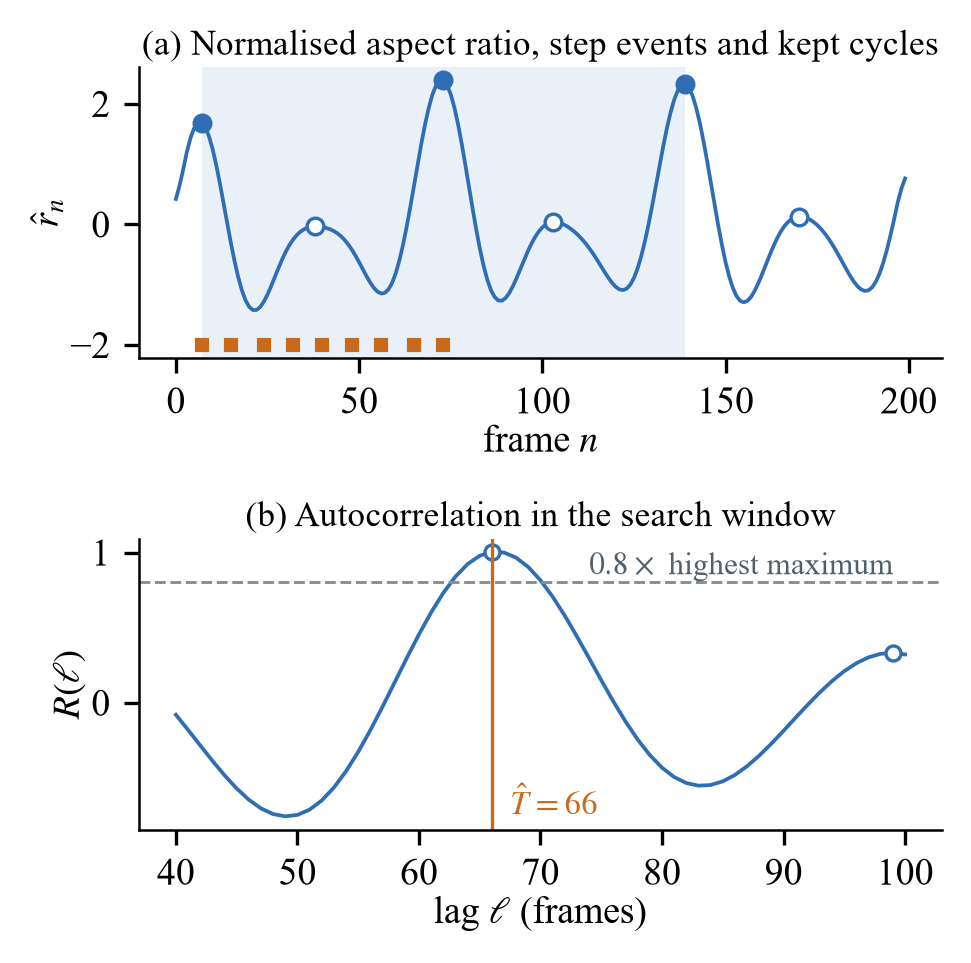
\includegraphics[width=\columnwidth]{fig_init_cycles.png}
\caption{INIT cycle detection (B1), run with the detector of the final code on a synthetic limping walk whose cycle lasts 66 frames. (a) The normalised aspect ratio $\hat{r}_n$ peaks at each double support, with large (filled) and small (open) peaks alternating. Of the four candidate cycles (event $i$ to event $i+2$), only the two that start on a large peak are kept (shaded); squares mark the nine phase frames (\ref{eq:phase}) of the first. (b) Autocorrelation (\ref{eq:acf}): $\hat{T}$ is the smallest local maximum (circles) that reaches 0.8 of the highest one.}
\label{fig:init}
\end{figure}

\textbf{Phase sampling.} B2 represents a cycle by nine phase frames $k_0,\dots,k_8$. On GAIT-IT these are the key frames of the block. On INIT they divide the detected cycle $[n_s,n_e]$ into eight equal parts,
\begin{equation}
k_t=\mathrm{round}\left(n_s+\frac{t}{8}(n_e-n_s)\right),\quad t=0,\dots,8.
\label{eq:phase}
\end{equation}
Both rules tie the samples to the cycle rather than to the clock. A person walking $\alpha$ times faster produces $x_\alpha(n)=x(\alpha n)$, with cycle boundaries $n_s/\alpha$ and $n_e/\alpha$, and (\ref{eq:phase}) then returns the same nine frames $x(k_t)$ for every $\alpha$, up to rounding to whole frames: rhythm is removed from the input. The GAIT-IT template behaves the same way, as it too places frames at fixed fractions of the cycle. Neither rule absorbs timing changes inside the cycle, such as a shortened stance on one side; those stay in the input as a change of pose at a given $t$, which is what the network reads.

\textbf{Phase jitter.} A phase frame may be off by a couple of frames. Each phase $t$ therefore keeps three candidate frames, $k_t+j$ with $j\in\{-2,0,+2\}$, clamped to the sequence. In training every phase draws its own offset at random; at test time three aligned views, with the same $j$ for all nine phases, are evaluated and averaged (Section~\ref{sec:infer}).

\textbf{Image input.} Each selected frame is cropped to the bounding box of its foreground (grey level above 30), enlarged by 8\,\% of the box height at the top and bottom and by 8\,\% of its width at the sides, within the frame. The crop is resized bilinearly with its aspect ratio kept, so that the longer side is 96 pixels, and centred on a black $96\times96$ canvas; frames of mirrored walks are flipped afterwards. GAIT-IT silhouettes touch the top and bottom of the frame, so there the vertical enlargement has no effect. With $\mathbf{x}_t\in[0,1]^{96\times96}$ the frame of phase $t$ and $\bar{\mathbf{x}}=\frac{1}{9}\sum_t\mathbf{x}_t$, the network input stacks three channels per phase,
\begin{equation}
\mathbf{X}=\left[2\mathbf{x}_t-1,\;\mathbf{x}_t-\mathbf{x}_{(t-1)\,\mathrm{mod}\,9},\;\mathbf{x}_t-\bar{\mathbf{x}}\right]_{t=0}^{8},
\label{eq:input}
\end{equation}
a tensor of size $3\times9\times96\times96$. The first channel is the silhouette; the second is its change since the previous phase, taken circularly so that phase 0 is compared to phase 8; and the third is its deviation from $\bar{\mathbf{x}}$, the gait energy image (GEI)~\cite{gei} of the cycle.

\subsection{Posture-geometry signals (input of B6)}
\label{sec:geom}

Cropping brings every frame to the same size. This keeps the shape of the silhouette in each frame, but it removes how the frames relate to each other: a change of body height over the cycle and the vertical bob of the body. We therefore measure posture on the recorded frame of each phase, before cropping, at the same jittered frames as the images (Fig.~\ref{fig:geom}). The frame is binarised (grey level above 127). Let $y_0$, $h$ and $w$ be the top row, the height and the width of the silhouette's bounding box, $c_x^{\mathrm{box}}$ the horizontal centre of the box, $(c_x,c_y)$ the centroid of the silhouette and $A$ its area in pixels. For a horizontal band covering the fractions $[a,b]$ of the box height, counted from the top, $w_{[a,b]}$ is the width of the silhouette within the band and $c_{x,[a,b]}$ the mean column of its pixels there. With $\tilde{h}$ and $\tilde{y}_0$ the medians of $h$ and $y_0$ over the sampled frames of the walk, and $\varsigma=-1$ for mirrored walks ($+1$ otherwise), Table~\ref{tab:geom} defines nine signals. An empty frame gives zeros.

\begin{table}[t]
\centering
\footnotesize
\caption{Posture-Geometry Signals of B6, Measured on Each Recorded Frame}
\label{tab:geom}
\begin{tabular}{clll}
\toprule
 & Signal & Definition & Reflects \\
\midrule
1 & Height$^{*}$ & $h/\tilde{h}-1$ & crouch, stoop \\
2 & Box width & $w/\tilde{h}$ & stride length \\
3 & Lower-body width & $w_{[0.70,1]}/\tilde{h}$ & foot separation \\
4 & Upper-body width & $w_{[0.15,0.55]}/\tilde{h}$ & arms, trunk \\
5 & Head bob$^{*}$ & $(y_0-\tilde{y}_0)/\tilde{h}$ & vertical bob \\
6 & Centroid height & $(c_y-y_0)/h$ & mass height \\
7 & Trunk lean & $\varsigma(c_{x,[0,0.3]}-c_{x,[0.7,1]})/\tilde{h}$ & lean \\
8 & Mass offset & $\varsigma(c_x-c_x^{\mathrm{box}})/\tilde{h}$ & mass shift \\
9 & Fill ratio & $A/(hw)$ & compactness \\
\bottomrule
\end{tabular}

\vspace{2pt}
\footnotesize $^{*}$ Constant on GAIT-IT and therefore not used there. Image rows grow downwards: signal 5 is positive when the head is below its median level, and signal 6 is the depth of the centroid below the top of the box.
\end{table}

\begin{figure}[t]
\centering
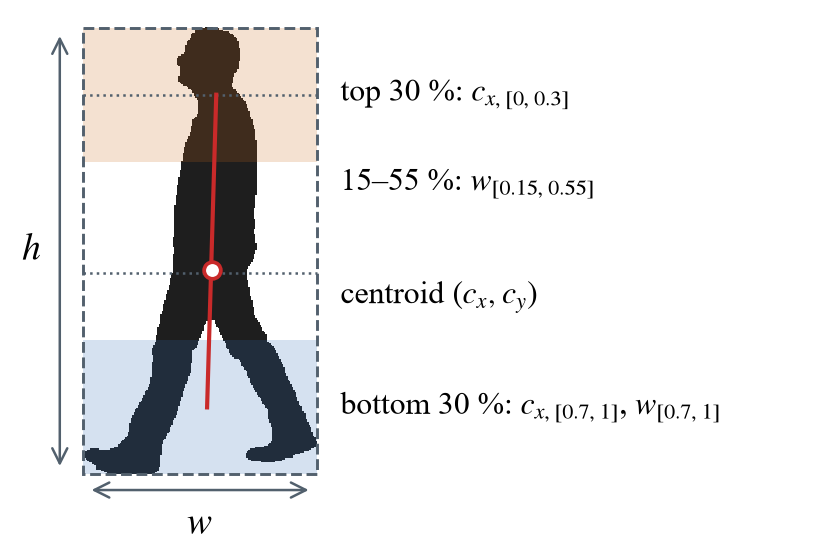
\includegraphics[width=\columnwidth]{fig_geometry.png}
\caption{Measurements behind Table~\ref{tab:geom}, drawn on one real INIT frame (normal walking, recorded moving right to left, so $\varsigma=-1$). Dashed: bounding box; shaded: the top and bottom 30\,\% bands; dotted: the 15--55\,\% band limits. The line joins the mean columns of the top and bottom bands (trunk lean), and the circle marks the centroid. With $\tilde{h}=323$ pixels for this walk, signals 1--9 of this frame are $-0.012$, $0.517$, $0.517$, $0.186$, $0.009$, $0.543$, $-0.020$, $-0.026$ and $0.319$.}
\label{fig:geom}
\end{figure}

\textbf{What each dataset provides.} The two datasets do not record the same thing. INIT frames are 800 pixels wide and 400 high, with the walker at its natural size and height; the box height changes within a walk, so all nine signals vary. GAIT-IT frames arrive already normalised to $224\times224$ pixels with the silhouette filling the height: $h=224$ and $y_0=0$ in every frame, so signals 1 and 5 are exactly zero in all cycles, and the recording holds no information on crouch or vertical bob. Signals that are constant over a dataset are dropped, which leaves $S=7$ signals on GAIT-IT and $S=9$ on INIT. On GAIT-IT the seven remaining signals describe the shape of the silhouette relative to its own height. The appearance stream can see this shape too, so here the geometry stream gives it in explicit form rather than adding unseen information.

The signals of a cycle form a matrix $\mathbf{G}\in\mathbb{R}^{9\times S}$ (phases $\times$ signals). Every signal is a ratio of two lengths or of two areas. A change of camera distance scales all lengths by one factor $\kappa$, which cancels, e.g., $\kappa h/(\kappa\tilde{h})=h/\tilde{h}$. Positions enter only as differences, so where the walker appears in the frame does not matter either. Because the measured frames are not mirrored, $\varsigma$ multiplies the two horizontal signals, so that their sign has the same meaning, forward or backward, in every walk.

\subsection{Network (B3--B8)}

Table~\ref{tab:params} lists the blocks with their output sizes and parameter counts.

\textbf{B3 -- (2+1)D backbone.} The backbone is the stem and layers 1--3 of an ImageNet-pretrained ResNet-18~\cite{resnet}, turned into a (2+1)D network~\cite{r2plus1d} over the nine phases. Every $k\times k$ convolution becomes a $1\times k\times k$ convolution and keeps its ImageNet weights and batch-norm statistics, as in the inflation of I3D~\cite{i3d}; with a temporal size of one, no weight has to be replicated. The three channels of (\ref{eq:input}) take the place of the RGB channels, and layer 4 is dropped, so that a $96\times96$ input still leaves a $6\times6$ map. Each residual block computes
\begin{equation}
\mathbf{u}=\mathrm{ReLU}\left(\mathrm{BN}_1(W_1*\mathbf{x})\right),
\end{equation}
\begin{equation}
\mathbf{v}=\mathrm{ReLU}\left(\mathbf{u}+\mathrm{BN}_t(W_t\circledast\mathbf{u})\right),
\end{equation}
\begin{equation}
\mathbf{y}=\mathrm{ReLU}\left(\mathrm{BN}_2(W_2*\mathbf{v})+S(\mathbf{x})\right),
\label{eq:block}
\end{equation}
where $W_1$ and $W_2$ are the pretrained $1\times3\times3$ convolutions, $S$ is the identity or the pretrained $1\times1\times1$ projection with its batch norm, and $W_t$ is a new $3\times1\times1$ convolution over the phase axis. It wraps around,
\begin{equation}
(W\circledast\mathbf{u})_t=\sum_{j=-1}^{1}W_j\,\mathbf{u}_{(t+j)\,\mathrm{mod}\,9},
\label{eq:circ}
\end{equation}
because completion is followed by the next initial contact, so no phase sits at an edge. The scale of $\mathrm{BN}_t$ starts at zero, so at initialization the temporal branch adds nothing and every block is its pretrained 2D counterpart, applied phase by phase; the temporal branch then learns motion on top. The stem ($1\times7\times7$ convolution and $1\times3\times3$ max pooling, both with spatial stride 2) and layers 1--3 output $64\times9\times24^2$, $64\times9\times24^2$, $128\times9\times12^2$ and $256\times9\times6^2$ maps; the phase axis is never strided. Of the 3.30\,M backbone parameters, 2.78\,M are initialised from ImageNet and 0.52\,M belong to the new temporal branches.

\textbf{B4 -- Body-part pooling.} Following GaitSet~\cite{gaitset}, we cut the $6\times6$ map of every phase into six horizontal strips, one row each, from head to feet, and add the whole map as a seventh, global part ($P=7$). Each part is average and max-pooled, the two 256-d vectors are concatenated, and a projection of its own, $\Theta_p\in\mathbb{R}^{512\times128}$, maps them to the phase feature $\mathbf{f}_{p,t}\in\mathbb{R}^{128}$.

\textbf{B5 -- Part temporal head.} Each part receives a learned phase embedding $\boldsymbol{\pi}_{p,t}$, initialized from $\mathcal{N}(0,0.02^2)$, and a residual circular temporal convolution with a kernel $V_p$ of its own (a grouped convolution, one group per part):
\begin{equation}
\mathbf{f}'_{p,\cdot}=\mathbf{f}_{p,\cdot}+\boldsymbol{\pi}_{p,\cdot},
\end{equation}
\begin{equation}
\mathbf{f}''_{p,\cdot}=\mathbf{f}'_{p,\cdot}+\mathrm{ReLU}\left(\mathrm{BN}(V_p\circledast\mathbf{f}'_{p,\cdot})\right).
\label{eq:part}
\end{equation}
Three summaries pool the nine phases of part $p$. Attention pooling uses a learned query $\mathbf{q}_p$, initialized to zero so that it starts as a plain average,
\begin{equation}
a_{p,t}=\mathrm{softmax}_t\left(\mathbf{q}_p^{\top}\mathbf{f}''_{p,t}\right),\quad \mathbf{f}^{\mathrm{att}}_p=\sum_{t=0}^{8}a_{p,t}\,\mathbf{f}''_{p,t};
\label{eq:att}
\end{equation}
max pooling gives $\mathbf{f}^{\max}_p=\max_t\mathbf{f}''_{p,t}$; and the half-cycle symmetry term is
\begin{equation}
\mathbf{s}_p=\frac{1}{4}\sum_{t=0}^{3}\left|\mathbf{f}''_{p,t}-\mathbf{f}''_{p,t+4}\right|.
\label{eq:sym}
\end{equation}
In a side view the other leg reaches the same pose about half a cycle later, so $\mathbf{s}_p\approx\mathbf{0}$ for a symmetric walker and grows with a one-sided impairment; phase 8, the end of the cycle, is left out. On GAIT-IT phase $t+4$ lies 48.0\,\% to 50.7\,\% of the stride after phase $t$ (Table~\ref{tab:phases}), which is close to half a cycle. The part descriptor is $[\mathbf{f}^{\mathrm{att}}_p\,\|\,\mathbf{f}^{\max}_p\,\|\,\mathbf{s}_p]\in\mathbb{R}^{384}$, and the seven descriptors are batch-normalized together into $\mathbf{g}^{\mathrm{app}}\in\mathbb{R}^{7\times384}$.

\textbf{B6 -- Geometry stream.} The posture matrix $\mathbf{G}$ is standardised signal by signal with batch normalisation and encoded by two circular temporal convolutions over the phases (kernel 3, 64 channels, each followed by batch normalisation and ReLU; the second is residual):
\begin{equation}
\mathbf{z}^{(1)}=\mathrm{ReLU}\left(\mathrm{BN}(U_1\circledast\mathrm{BN}(\mathbf{G}))\right),
\end{equation}
\begin{equation}
\mathbf{z}^{(2)}=\mathbf{z}^{(1)}+\mathrm{ReLU}\left(\mathrm{BN}(U_2\circledast\mathbf{z}^{(1)})\right).
\label{eq:geo}
\end{equation}
Mean pooling, max pooling and the symmetry term (\ref{eq:sym}), applied to $\mathbf{z}^{(2)}\in\mathbb{R}^{64\times9}$ and followed by batch normalisation, give the 192-d geometry feature $\mathbf{g}^{\mathrm{geo}}$.

\textbf{B7 -- Classifier ensemble.} The seven 384-d part slices of $\mathbf{g}^{\mathrm{app}}$ and the geometry feature $\mathbf{g}^{\mathrm{geo}}$ each have a linear classifier of their own, applied after dropout (rate 0.3). This gives eight logit vectors $\mathbf{z}_1,\dots,\mathbf{z}_8\in\mathbb{R}^{C}$, and the cycle scores are their average,
\begin{equation}
\mathbf{z}=\frac{1}{8}\sum_{i=1}^{8}\mathbf{z}_i,\quad \hat{y}=\arg\max_c z_c.
\label{eq:avg}
\end{equation}
Averaging lowers the variance of the decision whenever the errors of the classifiers are not perfectly correlated. The concatenation $\mathbf{g}=[\mathbf{g}^{\mathrm{app}}\,\|\,\mathbf{g}^{\mathrm{geo}}]\in\mathbb{R}^{2880}$ is the cycle descriptor of (\ref{eq:model}), read by the two heads below.

\textbf{Severity head.} A linear layer on $\mathbf{g}$, after dropout, predicts the severity $v\in\{\mathrm{normal},\mathrm{mild},\mathrm{severe}\}$ of the walk. GAIT-IT records each pathology at two levels: level 1 is labelled mild, level 2 severe, and normal walks normal. In six-class INIT, reduced arm swing at level 0.5 is mild, at level 0 severe, normal walking is normal, and the half-step and full-body walks carry no severity label. The head is an auxiliary task: it shapes $\mathbf{g}$ during training, and its output takes no part in the gait decision.

\textbf{B8 -- Walk head.} Each cycle descriptor is embedded as $\mathbf{e}_k=\mathrm{ReLU}(W_e\mathbf{g}_k+\mathbf{b}_e)\in\mathbb{R}^{256}$, with dropout on $\mathbf{g}_k$. For the $K$ cycles of a walk, in temporal order, B8 computes element-wise
\begin{equation}
\boldsymbol{\mu}=\frac{1}{K}\sum_{k=1}^{K}\mathbf{e}_k,
\end{equation}
\begin{equation}
\boldsymbol{\sigma}=\left(\frac{1}{K-1}\sum_{k=1}^{K}(\mathbf{e}_k-\boldsymbol{\mu})^2+\epsilon\right)^{1/2},
\end{equation}
\begin{equation}
\boldsymbol{\delta}=\frac{1}{K-1}\sum_{k=1}^{K-1}\left|\mathbf{e}_{k+1}-\mathbf{e}_k\right|,
\label{eq:walk}
\end{equation}
with $\epsilon=10^{-6}$; a walk of one cycle gets $\boldsymbol{\sigma}=\sqrt{\epsilon}$ and $\boldsymbol{\delta}=\mathbf{0}$. The walk is classified from $[\boldsymbol{\mu}\,\|\,\boldsymbol{\sigma}\,\|\,\boldsymbol{\delta}]\in\mathbb{R}^{768}$ by layer normalisation, dropout and a two-layer perceptron ($768\to128\to C$, ReLU). Here $\boldsymbol{\mu}$ describes the typical cycle, $\boldsymbol{\sigma}$ how much the cycles of the walk differ, and $\boldsymbol{\delta}$ how much they change from one stride to the next, i.e., the stride-to-stride difference that clinicians use as a marker. On INIT walks whose cycles overlap (Section~\ref{sec:cycles}), successive cycles start half a cycle apart, so there $\boldsymbol{\delta}$ follows step-to-step change.

\begin{table}[t]
\centering
\footnotesize
\caption{Blocks of the Final Model for GAIT-IT ($C=5$, $S=7$)}
\label{tab:params}
\begin{tabular}{llrr}
\toprule
Block & Operation & Output & Parameters \\
\midrule
Input & three channels, Eq. (\ref{eq:input}) & $3\times9\times96^2$ & -- \\
B3 stem & $1\times7\times7$ conv, max pool & $64\times9\times24^2$ & 9\,536 \\
B3 layer 1 & two (2+1)D blocks & $64\times9\times24^2$ & 172\,800 \\
B3 layer 2 & two (2+1)D blocks & $128\times9\times12^2$ & 624\,384 \\
B3 layer 3 & two (2+1)D blocks & $256\times9\times6^2$ & 2\,493\,952 \\
B4 & 7 parts, avg, max, $\Theta_p$ & $7\times9\times128$ & 458\,752 \\
B5 & $\boldsymbol{\pi}$, $V_p$, three poolings & $7\times384$ & 360\,192 \\
B6 & two circular convs, poolings & 192 & 14\,286 \\
B7 & eight linear classifiers & $8\times C$ & 14\,440 \\
Severity & linear (auxiliary) & 3 & 8\,643 \\
B8 & $\mathbf{e}_k$, statistics, MLP & $C$ & 838\,149 \\
Total & & & 4\,995\,134 \\
\bottomrule
\end{tabular}

\vspace{2pt}
\footnotesize Sizes are channels $\times$ phases $\times$ height $\times$ width. B6 grows with $S$, and B7 and B8 grow with $C$; on INIT ($C=6$, $S=9$) the total is 4\,998\,539.
\end{table}

\subsection{Training objective}

Every class loss is a focal loss~\cite{focal} with label smoothing~\cite{smoothing}. For scores $\mathbf{z}$, probabilities $\mathbf{p}=\mathrm{softmax}(\mathbf{z})$ and true class $y$, the smoothed target is $q_y=1-\varepsilon$ and $q_c=\varepsilon/(C-1)$ for $c\ne y$, and
\begin{equation}
\ell(\mathbf{z},y)=-\sum_{c=1}^{C}(1-p_c)^{\gamma}\,q_c\log p_c,
\label{eq:focal}
\end{equation}
with $\gamma=1.5$ and $\varepsilon=0.05$. The factor $(1-p_c)^{\gamma}$ lowers the weight of cycles that are already classified with confidence. The loss of a batch is
\begin{equation}
\mathcal{L}=\mathcal{L}_{\mathrm{focal}}+0.5\,\mathcal{L}_{\mathrm{part}}+0.3\,\mathcal{L}_{\mathrm{sev}}+\mathcal{L}_{\mathrm{walk}},
\label{eq:loss}
\end{equation}
with
\begin{equation}
\mathcal{L}_{\mathrm{focal}}=\langle\ell(\mathbf{z},y)\rangle,\quad \mathcal{L}_{\mathrm{part}}=\frac{1}{8}\sum_{i=1}^{8}\langle\ell(\mathbf{z}_i,y)\rangle,
\label{eq:parts}
\end{equation}
where $\langle\cdot\rangle$ is the mean over the cycles of the batch. $\mathcal{L}_{\mathrm{focal}}$ trains the averaged scores (\ref{eq:avg}), and $\mathcal{L}_{\mathrm{part}}$ trains each of the eight classifiers on its own, so that every body part, and the geometry stream, must be discriminative by itself. $\mathcal{L}_{\mathrm{sev}}$ is the plain cross-entropy of the severity head over the cycles that carry a severity label. $\mathcal{L}_{\mathrm{walk}}$ applies (\ref{eq:focal}) to the walk scores $\hat{\mathbf{z}}$ of the walk samples in the batch (Section~\ref{sec:batch}).

\subsection{Batches, augmentation and optimisation}
\label{sec:batch}

\textbf{Walk-based batches.} Each optimisation step draws $K$ uniformly from $\{2,\dots,6\}$ and then $\lfloor16/K\rfloor$ training walks, with replacement and with a probability proportional to $n_c^{-1/2}$, where $n_c$ is the number of training walks in the walk's class. A class is thus drawn in proportion to $\sqrt{n_c}$, which softens the class imbalance without removing it. From each drawn walk, $K$ consecutive cycles are taken from a random start; a shorter walk contributes all its cycles, and the empty slots, filled with copies of its first cycle, are masked out of the losses and of the walk statistics. These copies still pass through the network, so they do enter the batch-norm statistics of that step. A batch therefore holds at most 16 cycles. The cycle terms of (\ref{eq:loss}) use all of them, and $\mathcal{L}_{\mathrm{walk}}$ uses the $\lfloor16/K\rfloor$ walk samples, so the walk head learns from walks of up to six cycles. One epoch is $\lfloor N_{\mathrm{tr}}/16\rfloor$ steps, with $N_{\mathrm{tr}}$ the number of training cycles.

\textbf{Augmentation.} Only training batches are augmented (Table~\ref{tab:settings}). Besides the phase jitter of Section~\ref{sec:cycles}, each cycle receives one random rotation (up to $\pm5^\circ$), scaling (up to $\pm8$\,\%) and translation (up to $\pm2.4$ pixels), applied identically to its nine phases. With probability 0.15 each, the whole cycle is dilated or eroded with a $3\times3$ window, which acts like segmentation errors, and with probability 0.2 one rectangle of 6--16 pixels per side is erased~\cite{erasing} at the same place in all nine phases. All of this acts on $\mathbf{x}_t$ before the channels of (\ref{eq:input}) are formed, so the motion and GEI channels stay consistent with the silhouettes. The posture matrix $\mathbf{G}$ is multiplied by one random gain in $[0.95,1.05]$ per cycle and receives Gaussian noise of 0.05 standard deviations of each signal, the deviations being taken over the training cycles of the fold.

\textbf{Optimisation.} AdamW~\cite{adamw}, with weight decay 0.05 on all parameters, updates two parameter groups: the backbone B3 with a peak learning rate of $3\times10^{-4}$, and all other layers with $10^{-3}$. Both follow a one-cycle schedule~\cite{onecycle} over the whole run: the rate rises along a cosine from 1/25 of its peak to the peak during the first 15\,\% of the steps, then falls along a cosine to $1/(25\cdot10^4)$ of the peak, while Adam's $\beta_1$ moves the opposite way between 0.95 and 0.85. Gradients are clipped to a global $\ell_2$ norm of 2, and mixed-precision (FP16) arithmetic with loss scaling keeps training within 4\,GB of GPU memory. After every step, an exponential moving average (EMA) of all weights and batch-norm statistics is updated, $\bar{\theta}\leftarrow0.98\,\bar{\theta}+0.02\,\theta$; the averaged weights are the ones that are evaluated. Training always runs for 20 epochs, and Algorithm~\ref{alg:fold} summarizes one fold.

\begin{table}[t]
\centering
\footnotesize
\caption{Training and Test Settings of the Final Model}
\label{tab:settings}
\begin{tabular}{ll}
\toprule
Setting & Value \\
\midrule
Batch & $\lfloor16/K\rfloor$ walks $\times$ $K$ cycles, $K\sim U\{2,\dots,6\}$ \\
Walk sampling & $P(\mathrm{walk})\propto n_c^{-1/2}$ (square-root balance) \\
Training length & 20 epochs of $\lfloor N_{\mathrm{tr}}/16\rfloor$ steps, no early stopping \\
Optimiser & AdamW, weight decay 0.05 (all parameters) \\
Peak learning rate & $10^{-3}$ (heads), $3\times10^{-4}$ (backbone B3) \\
Schedule & one-cycle, 15\,\% warm-up, cosine shape \\
Rate range & peak/25 $\to$ peak $\to$ peak$/(25\cdot10^4)$ \\
Adam $\beta_1$ & $0.95\to0.85\to0.95$ (against the rate) \\
Gradient clipping & global $\ell_2$ norm 2 \\
Precision & FP16 mixed precision \\
Weight averaging & EMA, decay 0.98, after every step \\
Loss & Eq. (\ref{eq:loss}); $\gamma=1.5$, $\varepsilon=0.05$ \\
Dropout & 0.3 in all heads \\
Phase jitter & offset $j\in\{-2,0,+2\}$ frames, drawn per phase \\
Spatial augmentation & rotation $\pm5^\circ$, scale $\pm8$\,\%, shift $\pm2.4$ px \\
Segmentation noise & $3\times3$ dilation or erosion, $p=0.15$ each \\
Random erasing & $p=0.2$; 6--16 px box, same in all phases \\
Geometry augmentation & gain $1\pm0.05$; noise $0.05\sigma$ per signal \\
Test time & EMA weights of epoch 20; 3 jitter views averaged \\
Seeds & 42 (folds); 42 (training, set once for all folds) \\
Hardware & RTX 3050 Laptop GPU, 4\,GB \\
\bottomrule
\end{tabular}
\end{table}

\begin{algorithm}[t]
\caption{Training and testing in one fold}
\label{alg:fold}
\begin{algorithmic}[1]
\Require training, monitoring and test walks of fold $k$
\State B3 $\leftarrow$ inflated ResNet-18 (ImageNet); $\gamma(\mathrm{BN}_t)\leftarrow0$; $\bar{\theta}\leftarrow\theta$
\State noise scale of $\mathbf{G}$ $\leftarrow$ deviations over the training cycles
\For{$s=1,\dots,20\lfloor N_{\mathrm{tr}}/16\rfloor$}
\State $K\sim U\{2,\dots,6\}$; draw $\lfloor16/K\rfloor$ walks, $P\propto n_c^{-1/2}$
\State take $K$ consecutive cycles per walk; mask empty slots
\State draw an offset $j$ per phase; augment images and $\mathbf{G}$
\State compute $\mathbf{z}_1,\dots,\mathbf{z}_8$, $\mathbf{z}$, severity, $\mathbf{e}_k$ and $\hat{\mathbf{z}}$
\State AdamW step on $\mathcal{L}$ (\ref{eq:loss}), one-cycle rate, $\|\nabla\|_2\le2$
\State $\bar{\theta}\leftarrow0.98\,\bar{\theta}+0.02\,\theta$
\State after each epoch: log $\bar{\theta}$ on the monitoring group
\EndFor
\State test $\bar{\theta}$: 3 jitter views per cycle; B8 on all cycles of a walk
\end{algorithmic}
\end{algorithm}

\subsection{Inference}
\label{sec:infer}

The test model is the EMA of the last epoch; no epoch or checkpoint is selected. Each test cycle is evaluated in the three aligned jitter views of Section~\ref{sec:cycles}, and its scores $\mathbf{z}$ and its embedding $\mathbf{e}$ are averaged over the views. The cycle class follows (\ref{eq:avg}). The walk class comes from B8 applied to all cycles of the walk, in temporal order, however many there are: up to 13 on GAIT-IT and 17 on INIT, although training sees at most six. As a reference that needs no walk head, the soft vote averages the log-probabilities of the $M$ cycles of a walk,
\begin{equation}
\hat{y}_{\mathrm{vote}}=\arg\max_c\frac{1}{M}\sum_{m=1}^{M}\log\mathrm{softmax}(\mathbf{z}_m)_c.
\label{eq:vote}
\end{equation}

\subsection{Evaluation methodology}
\label{sec:eval}

\textbf{Subject-exclusive folds.} The subject IDs are sorted, shuffled with a fixed seed (Python's \texttt{random.Random(42)}) and dealt round-robin into ten groups. On GAIT-IT the 23 subjects form three groups of three and seven groups of two; on INIT each of the ten subjects is a group of its own. Fold $k$ tests on group $k$, monitors training on group $k+1$ (group 1 for $k=10$) and trains on the remaining eight groups. Every subject is tested exactly once, and no subject has two roles in one fold; the code stops if this is ever violated. A walk is one recorded sequence, identified by its gait class, subject and name, and the code also stops if a walk would mix labels or subjects.

The monitoring group is evaluated after every epoch for the training curves only. Within a run, with a fixed number of epochs and the last weights tested, no model or epoch is chosen on monitoring or test subjects. The settings of Table~\ref{tab:settings} and the choice of the final variant, however, come from earlier versions that were compared on these same ten folds, so the test folds are not fully untouched by model development. All variants share the folds, the training seed and the settings of Table~\ref{tab:settings}.

\textbf{Metrics.} For each fold, cycle accuracy is the share of test cycles with $\hat{y}=y$, and macro-F1 is the mean over the classes of $2P_cR_c/(P_c+R_c)$, with $P_c$ and $R_c$ the precision and recall of class $c$. Walk accuracy and walk macro-F1 are computed in the same way over the test walks. Macro-F1 averages over all $C$ classes, an undefined F1 counting as zero; every class is present in every test fold of both datasets. Severity accuracy is the share of correctly graded test cycles among those with a severity label. Each metric is reported as mean $\pm$ population standard deviation over the ten folds. Per-class recall is read from the cycle-level confusion matrix summed over the ten test folds, and the spread across folds shows how much a result depends on who is in the test group.

\textbf{Ablations.} Each component can be removed on its own while everything else stays fixed: the geometry stream (B6); the walk head (B8), in which case walks are decided by the soft vote (\ref{eq:vote}) and batches are drawn cycle by cycle, with square-root balancing over cycles; the severity task; and the symmetry term of B5 (B6 always keeps its own). The (2+1)D backbone can also be replaced by the same ResNet-18 applied to each phase in 2D, with a cyclic temporal shift~\cite{tsm} of one eighth of the channels in each direction, which adds no parameters.

\textbf{Subject-adversarial variant.} To test whether removing subject identity from $\mathbf{g}$ helps, a subject classifier ($2880\to128\to$ one output per subject) is attached to $\mathbf{g}$ through a gradient-reversal layer~\cite{dann}. The layer passes $\mathbf{g}$ forward unchanged and multiplies its gradient by $-\lambda(\rho)$, with
\begin{equation}
\lambda(\rho)=0.1\left(\frac{2}{1+e^{-10\rho}}-1\right),
\label{eq:lambda}
\end{equation}
where $\rho\in[0,1]$ is the fraction of training completed. The subject cross-entropy is added to (\ref{eq:loss}) with weight 1. The final model does not use this variant.

\textbf{Implementation.} The model is written in PyTorch. It has 4\,995\,134 trainable parameters on GAIT-IT and 4\,998\,539 on INIT. Training and testing run on one RTX 3050 Laptop GPU with 4\,GB of memory.

\subsection{Changes from version 6}
\label{sec:changes}

Version 7 keeps the architecture, the losses and the settings of version 6, and it corrects the data handling.

\textbf{Cycle reading.} Version 6 advanced through the GAIT-IT key-frame lists by eight entries instead of nine. Only 851 of its 3813 cycles started at $t=0$; the other 2962 were shifted in phase and held a repeated frame. Version 7 reads whole blocks and has 3783 cycles.

\textbf{Walk identity.} Subject s9's hemiplegic recordings are named \texttt{s9pat1*}, like the same subject's diplegic ones. Version 6 identified a walk by subject and name, so eight pairs of recordings became eight mixed-class walks, leaving 813 walks. The identity now includes the class, which gives 821 walks.

\textbf{Geometry signals.} Height and head bob, constant on GAIT-IT, are dropped there, which removes 388 parameters. The noise scale of the geometry augmentation now comes from the training cycles of each fold instead of from the whole dataset.

\textbf{Crop.} The crop box now includes its last row and column, so the enlargement is equal on both sides, and the resized side is rounded rather than truncated.

\begin{thebibliography}{99}
\bibitem{gaitit} P. Albuquerque, J. P. Machado, T. T. Verlekar, P. L. Correia, and L. D. Soares, ``Remote gait type classification system using markerless 2D video,'' \emph{Diagnostics}, vol. 11, no. 10, p. 1824, 2021.
\bibitem{init} J. Ortells, M. T. Herrero-Ezquerro, and R. A. Mollineda, ``Vision-based gait impairment analysis for aided diagnosis,'' \emph{Med. Biol. Eng. Comput.}, vol. 56, no. 9, pp. 1553--1564, 2018.
\bibitem{perry} J. Perry and J. M. Burnfield, \emph{Gait Analysis: Normal and Pathological Function}, 2nd ed. Thorofare, NJ, USA: SLACK, 2010.
\bibitem{gei} J. Han and B. Bhanu, ``Individual recognition using gait energy image,'' \emph{IEEE Trans. Pattern Anal. Mach. Intell.}, vol. 28, no. 2, pp. 316--322, 2006.
\bibitem{resnet} K. He, X. Zhang, S. Ren, and J. Sun, ``Deep residual learning for image recognition,'' in \emph{Proc. IEEE CVPR}, 2016, pp. 770--778.
\bibitem{r2plus1d} D. Tran, H. Wang, L. Torresani, J. Ray, Y. LeCun, and M. Paluri, ``A closer look at spatiotemporal convolutions for action recognition,'' in \emph{Proc. IEEE CVPR}, 2018, pp. 6450--6459.
\bibitem{i3d} J. Carreira and A. Zisserman, ``Quo vadis, action recognition? A new model and the Kinetics dataset,'' in \emph{Proc. IEEE CVPR}, 2017, pp. 6299--6308.
\bibitem{gaitset} H. Chao, Y. He, J. Zhang, and J. Feng, ``GaitSet: Regarding gait as a set for cross-view gait recognition,'' in \emph{Proc. AAAI}, 2019, pp. 8126--8133.
\bibitem{focal} T.-Y. Lin, P. Goyal, R. Girshick, K. He, and P. Doll\'ar, ``Focal loss for dense object detection,'' in \emph{Proc. IEEE ICCV}, 2017, pp. 2980--2988.
\bibitem{smoothing} C. Szegedy, V. Vanhoucke, S. Ioffe, J. Shlens, and Z. Wojna, ``Rethinking the Inception architecture for computer vision,'' in \emph{Proc. IEEE CVPR}, 2016, pp. 2818--2826.
\bibitem{erasing} Z. Zhong, L. Zheng, G. Kang, S. Li, and Y. Yang, ``Random erasing data augmentation,'' in \emph{Proc. AAAI}, 2020, pp. 13001--13008.
\bibitem{adamw} I. Loshchilov and F. Hutter, ``Decoupled weight decay regularization,'' in \emph{Proc. ICLR}, 2019.
\bibitem{onecycle} L. N. Smith and N. Topin, ``Super-convergence: Very fast training of neural networks using large learning rates,'' in \emph{Proc. SPIE}, vol. 11006, 2019, Art. no. 1100612.
\bibitem{tsm} J. Lin, C. Gan, and S. Han, ``TSM: Temporal shift module for efficient video understanding,'' in \emph{Proc. IEEE ICCV}, 2019, pp. 7083--7093.
\bibitem{dann} Y. Ganin and V. Lempitsky, ``Unsupervised domain adaptation by backpropagation,'' in \emph{Proc. ICML}, 2015, pp. 1180--1189.
\end{thebibliography}

\vspace{6mm}
\noindent Signature of Supervisor: Prof. Samit Ari\\[2mm]
Date:

\end{document}
